\documentclass{article}
\usepackage{iclr2027_conference,times}
\input{math_commands.tex}
\usepackage{hyperref}
\usepackage{url}
\usepackage{booktabs}
\usepackage{graphicx}
\usepackage{multirow}
\usepackage[table]{xcolor}
\usepackage{amsmath}

% Numbers still to be re-read from regenerated tables (analyze_results.py). Remove before submission.
\newcommand{\vnum}[1]{\textcolor{red}{#1}}
\newcommand{\todo}[1]{\textcolor{blue}{[TODO: #1]}}

\title{Forgetting Has an Address: Output-Localised, Architecture-General, and Conserved Forgetting in Continual Document Understanding}

% Anonymous for submission (\iclrfinalcopy stays commented out).
\author{Anonymous authors\\Paper under double-blind review}

%\iclrfinalcopy
\begin{document}
\maketitle

\begin{abstract}
Continual-learning (CL) methods are developed almost exclusively on unimodal classification and treat the network as a homogeneous block. We ask what forgetting actually looks like inside a multimodal document encoder performing continual key-information extraction, and whether standard remedies act on it. Using per-group Fisher displacement and layer-wise CKA across four backbones (LayoutLMv3, LiLT, BROS, BERT), three scenarios (domain-, class-, and mixed-incremental) and three seeds, we find that forgetting is \emph{output-localised}---it concentrates in the shared classifier head and late encoder layers while input encoders stay nearly stable---and \emph{architecture-general}: the naive-to-joint gap agrees to within 2.5 points across all four backbones. Protecting the locus does not remove forgetting: freezing the head and late layers migrates the drift into early layers (CKA $1.00\rightarrow0.19$) with no change in accuracy, i.e.\ forgetting is \emph{conserved} under architectural constraint. This anatomy predicts, and our benchmark confirms, that only mechanisms which re-ground the head recover old competence: replay (ER, DER++) reaches the joint bound on domain-incremental learning ($\approx$88 vs.\ 88.7 average F1), regularisation and distillation stay at the naive floor (41--44), and a remedy's benefit is backbone-dependent (EWC ranges from $-12$ to $+5$ points). We then try to break the prediction with five buffer-free consolidation families---weight merging, subspace transfer, parametric slot memories, input-anchored memory, and feature-Gaussian generative replay---and each fails for the same identified reason: nothing they store reproduces replay's gradient on the head. A constructive control isolates what a buffer must contain: per-document SVD replay is lossless at $2.7\times$ compression, whereas every marginal or per-class summary collapses, with +27 points attributable to whole-document consistency alone. For document understanding the question is therefore not how to avoid the buffer, but how small it can be and what it must hold.
\end{abstract}

\section{Introduction}
\label{sec:intro}

Organisations process a continuous stream of visually-rich documents---forms, invoices, receipts, contracts---whose meaning depends not only on the words but on where those words sit on the page. Key-information extraction (KIE) from such documents is cast as token-level sequence labelling over a tri-modal input (OCR text, 2-D layout, page image), and multimodal document encoders such as LayoutLMv3~\citep{huang2022layoutlmv3}, LiLT~\citep{wang2022lilt} and BROS~\citep{hong2022bros} define the state of the art. Deployed systems are not static: new document types appear, schemas are extended, and the input distribution drifts, while retraining on all history is blocked by cost and by privacy constraints on the earlier data. This is continual learning (CL), and its central obstacle is catastrophic forgetting~\citep{mccloskey1989catastrophic}.

The CL literature offers a mature toolbox---importance-weighted regularisation~\citep{kirkpatrick2017ewc}, distillation from past models~\citep{li2017lwf}, exemplar replay~\citep{rolnick2019er,buzzega2020der}, task prompts~\citep{wang2022l2p,wang2022dualprompt,smith2023coda} and per-task low-rank adapters~\citep{wang2023olora}---but almost all of it was developed on unimodal image or text classification, and it treats the network as one homogeneous block: a single quadratic penalty across all parameters, whole-network output matching, or a depth-wise freezing cut chosen by hand. A tri-modal document encoder is manifestly \emph{not} homogeneous. It contains a text stream, a visual stream, layout embeddings, shared attention blocks at increasing depth, and a task head, trained on different signals with different inductive biases. The modern parameter-efficient and modular families do not resolve this; they sharpen it, because deciding \emph{which} weights to adapt or \emph{where} to inject a prompt presupposes knowing which part of the encoder is at risk.

\paragraph{Problem.} Under continual token-level KIE---a domain-incremental sequence over FUNSD, SROIE and CORD, a class-incremental split of CORD, and a mixed sequence that alternates the two---\emph{where} does forgetting occur inside a multimodal document encoder, is that location a property of the task or of the architecture, and which remedies act on it? We answer five questions in order.
\begin{enumerate}
  \item[\textbf{Q1}] \emph{Anatomy.} Which parameter groups drift, measured by per-group Fisher displacement and layer-wise CKA, and is the answer backbone-invariant?
  \item[\textbf{Q2}] \emph{Conservation.} Does protecting the drifting locus remove forgetting, or relocate it?
  \item[\textbf{Q3}] \emph{Prediction.} Does the anatomy predict the ordering of standard remedies, and does that ordering hold across backbones and scenarios?
  \item[\textbf{Q4}] \emph{Falsification.} Can any buffer-free mechanism substitute for the gradient that replay places on the head?
  \item[\textbf{Q5}] \emph{Buffer content.} If a buffer is necessary, what is the minimal thing it must contain?
\end{enumerate}

\paragraph{Findings.} Forgetting is \emph{output-localised}: the head carries more than an order of magnitude more Fisher importance than any other group and CKA drift rises monotonically with depth, from $1.00$ at the input encoders to $0.25$ at the late layers and $0.16$ at the head, while a controlled cross-condition test cannot distinguish the full multimodal model from its unimodal ablations (Q1, \S\ref{sec:anatomy}). It is \emph{architecture-general}: the same locus appears on LayoutLMv3, LiLT, BROS and text-only BERT, and the naive-to-joint gap agrees to within 2.5 points across the four (Q1). It is \emph{conserved}: freezing the head and late layers drives early-layer CKA from $1.00$ to $0.19$ at unchanged accuracy, and a no-memory control is indistinguishable, so drift---not memory---is the bottleneck (Q2). The anatomy predicts the remedy ordering: replay re-grounds the head and reaches the joint bound on domain-incremental learning, regularisation and distillation stay at the floor, and a remedy's benefit flips sign across backbones (Q3, \S\ref{sec:benchmark}). Five buffer-free families we built or ported all fail, and for one reason (Q4, \S\ref{sec:falsification}). Finally, a compressed per-document replay is lossless at $2.7\times$ while every marginal summary collapses, isolating whole-document consistency as the necessary ingredient (Q5, \S\ref{sec:buffer}).

\paragraph{Contributions.}
\begin{enumerate}
  \item A multi-backbone, multi-scenario, multi-seed \emph{anatomy} of forgetting in document IE: output-localised, architecture-general, and migrating under constraint.
  \item A prediction-tested benchmark of six classical CL methods across four backbones and three scenarios, showing that replay re-grounds the head and reaches the joint bound, that buffer-free remedies do not, and that remedy benefit is backbone-dependent.
  \item A convergent negative result over five buffer-free consolidation families with a single mechanistic explanation, and a constructive control isolating whole-document consistency as the necessary buffer ingredient.
\end{enumerate}
No method in this paper is proposed as a contribution; every method is evidence. The implication for document CL is a reframing of the research question from ``how to avoid the buffer'' to ``how small can it be, and what must it hold''.

\section{Related Work}
\label{sec:related}
\paragraph{Continual-learning families.} Following \citet{wang2024survey}, remedies fall into regularisation (EWC~\citep{kirkpatrick2017ewc}, SI~\citep{zenke2017si}, MAS~\citep{aljundi2018mas}; output-side distillation, LwF~\citep{li2017lwf}), replay (GEM~\citep{lopezpaz2017gem}, ER~\citep{rolnick2019er}, DER++~\citep{buzzega2020der}, iCaRL~\citep{rebuffi2017icarl}), optimisation-geometry (GPM~\citep{saha2021gpm}, OGD~\citep{farajtabar2020ogd}, C-Flat~\citep{bian2024cflat}), representation-based methods over a frozen backbone (L2P~\citep{wang2022l2p}, DualPrompt~\citep{wang2022dualprompt}, CODA-Prompt~\citep{smith2023coda}, O-LoRA~\citep{wang2023olora}, CL-LoRA~\citep{he2025cllora}, RanPAC~\citep{mcdonnell2023ranpac}), and architecture-based isolation~\citep{mallya2018packnet,yoon2018den}. Replay is empirically the strongest family~\citep{masana2022class,wang2024survey} but stores raw data, which is precisely what document deployments cannot keep. The buffer-free alternatives we test in \S\ref{sec:falsification} are drawn from the strongest current members of each line: model merging with classifier realignment (LCA~\citep{lca2026}), subspace transfer, and exemplar-free \emph{feature} replay---class-conditional Gaussians in a frozen feature space---which is the field's most successful buffer-free tool (PASS, FeTrIL, FeCAM~\citep{zhu2021pass,petit2023fetril,goswami2023fecam}).

\paragraph{Where forgetting lives.} \citet{ramasesh2021anatomy} localise forgetting in split image-classification tasks by resetting or freezing blocks of layers and find it concentrated in the deeper layers nearest the output; \citet{zhai2023investigating} show the same picture carries over to multimodal LLMs used as classifiers. Multimodal CL benchmarks add hints that architecture shapes forgetting---dual-stream models forget less than single-stream ones and deeper layers forget more~\citep{zhang2025clcrossvqa}---and per-layer budget routing (D-MoLE~\citep{ge2025dmole}) implicitly assumes non-uniform need without measuring it. None of these attributes forgetting to the components of a single tri-modal encoder, tests whether the location is architecture-invariant, or asks what happens to the drift when the located component is protected. We take the checkpoint-pair, per-layer stance of \citet{ramasesh2021anatomy} and extend it along two axes---component and backbone---and add the protection/migration experiment.

\paragraph{Continual information extraction.} Continual NER confronts the semantic shift of the ``O'' tag with distillation and pseudo-labelling (CPFD~\citep{zhang2023cpfd}, CFNER~\citep{zheng2022cfner}, ICE~\citep{liu2023ice}, SpanKL~\citep{zheng2023spankl}) or by generating spans (GenCNER~\citep{gencner}); continual RE pairs episodic memory with relation prototypes (EMAR~\citep{han2020emar}, RP-CRE~\citep{cui2021rpcre}, CRL~\citep{zhao2022crl}) or uses prompt pools under task-incremental assumptions (WAVE-CRE~\citep{le2025wavecre}). All are sentence-level and text-only. Document-level CL is nascent: GDI-Bench~\citep{gdibench} shows an MLLM forgets under fine-tuning and mitigates it by \emph{heuristic} layer freezing; continual table detection~\citep{minouei2022table} uses plain ER; ProtoNER~\citep{kumar2024protoner} reaches LayoutLM-family encoders only in a few-shot regime. No prior work diagnoses which component of a document encoder forgets, and none evaluates the classical CL families on multimodal KIE under one protocol across backbones.

\section{Setup}
\label{sec:setup}
\paragraph{Task.} A document is a triple $D=(W,B,I)$ of OCR tokens, normalised bounding boxes and the page image; the model $f_\theta$ emits BIO labels per token and is trained with token-level cross-entropy. Performance is entity-level F1 with BIO-aware span matching (\texttt{seqeval}). In the continual setting the learner sees tasks $\mathcal{T}_1,\dots,\mathcal{T}_T$ and at task $t$ may access only $\mathcal{D}_t$ and, for replay methods, a bounded memory. OCR and boxes are dataset-provided throughout, so no OCR engine enters the loop.

\paragraph{Datasets and scenarios.} We use FUNSD (149/50 train/test forms, 7 BIO tags), CORD (800/100/100 receipts, 30 fine-grained classes, 61 tags) and SROIE (626/347 receipts, 9 tags). \textbf{DIL}: FUNSD$\rightarrow$SROIE$\rightarrow$CORD under a fixed unified schema \{HEADER, KEY, VALUE, OTHER\}; the label space is constant and only the input distribution shifts, so forgetting is pure representation drift. \textbf{CIL-CORD}: CORD's 30 classes introduced six at a time over five sessions in a fixed easy-to-hard curriculum; the head grows, and tokens of not-yet-introduced classes are absorbed into ``O'', whose meaning therefore shifts. \textbf{Mixed}: a six-session sequence alternating new-class transitions within CORD with new-domain transitions to FUNSD and SROIE, ending in a FUNSD revisit. Session details and the DIL mapping are in Appendix~\ref{app:setup}.

\paragraph{Backbones.} LayoutLMv3-base~\citep{huang2022layoutlmv3} is the primary tri-modal encoder (text, layout, image; single-stream). LiLT-base~\citep{wang2022lilt} and BROS-base~\citep{hong2022bros} are layout-aware but vision-free; BERT-base is a text-only external comparator. Every method runs unchanged on all four through a shared wrapper contract (head expansion, parameter groups, gradient checkpointing); heads are plain linear layers.

\paragraph{Methods.} The generality grid covers the six classical strategies---naive sequential fine-tuning (lower bound), joint multi-task training on the pooled data (oracle upper bound), EWC, LwF, ER and DER++---on every backbone and scenario. Defaults: EWC $\lambda{=}10^3$ with Fisher over 200 samples; LwF $T{=}2$; ER/DER++ buffer of 200 documents, DER++ $\alpha{=}\beta{=}0.5$. The falsified buffer-free families of \S\ref{sec:falsification} and the compressed-replay controls of \S\ref{sec:buffer} run on LayoutLMv3/DIL unless stated. Prompt- and LoRA-based baselines (CODA-Prompt, O-LoRA, CL-LoRA, ER+C-Flat++) are reported in Appendix~\ref{app:extra}.

\paragraph{Protocol.} AdamW, learning rate $5\times10^{-5}$ constant, weight decay $0.01$, gradient clipping $1.0$. Each task trains \emph{to convergence}: early stopping on the task's validation entity-F1 with patience 2 and $\delta{=}0.1$ under a 100-epoch ceiling that never binds, restoring the best-validation checkpoint at each boundary. The identical rule applies to every method and session, replacing a fixed-budget protocol that systematically under-trained slow-converging methods (EWC in particular). FUNSD and SROIE ship no validation split; for them the stopping signal is read from the evaluation set, a mild optimistic bias shared identically by all methods and disclosed rather than hidden. Grid results are mean $\pm$ s.d.\ over seeds $\{42,7,123\}$.

\paragraph{Metrics.} From the accuracy matrix $R[i,j]$ (F1 on task $j$ after training task $i$) we report average accuracy $\mathrm{AA}=\frac{1}{T}\sum_j R[T,j]$, backward transfer $\mathrm{BWT}=\frac{1}{T-1}\sum_{j<T}(R[T,j]-R[j,j])$ and average forgetting $\mathrm{AF}=-\mathrm{BWT}$. We do not report forward transfer: under class-incremental label growth the zero-shot term is $\approx-85$ for every method and carries no information.

\paragraph{Diagnostics.} Two instruments localise forgetting. (i) \emph{Per-token linear CKA}~\citep{kornblith2019similarity} between the checkpoints before and after a task, at six depth-matched probe points (embeddings, patch embedding, early/mid/late encoder layers, classifier), computed over up to 2000 distinct valid tokens so the estimate is above the hidden width. (ii) \emph{Old-task-Fisher-weighted displacement} per parameter group,
\begin{equation}
  D_g=\sum_{\phi\in g} F^{(t-1)}_\phi\bigl(\theta^{(t)}_\phi-\theta^{(t-1)}_\phi\bigr)^2 ,
\end{equation}
which is large exactly where parameters that mattered for the previous task have been overwritten. We separate this from Fisher \emph{importance} $F_g$, which is largest at the head for any token classifier by the geometry of the output layer and is never labelled forgetting. Groups are the ones the architecture actually separates---text, layout and patch embeddings, shared attention, feed-forward/normalisation, and the head---plus depth buckets (input/early/mid/late/head).

\section{Anatomy of Forgetting}
\label{sec:anatomy}
\paragraph{Forgetting is total within one boundary, on every backbone.} Under naive sequential fine-tuning (FUNSD$\rightarrow$CORD$\rightarrow$SROIE, three seeds) the diagonal of $R$ is strong and the sub-diagonal collapses to 1--3 F1: LayoutLMv3 loses FUNSD from $89.1$ to $3.3$ after a single further task, LiLT $83.9\rightarrow2.1$, BROS $88.9\rightarrow6.6$; text-only BERT is the mildest (CORD held at $18.4$) but still loses most of each earlier task. On the DIL grid the naive floor is $41.3/40.1/40.3/39.4$ AA on LayoutLMv3/LiLT/BROS/BERT and the joint oracle $88.7/83.8/87.5/77.2$; on Mixed the joint-to-naive gap is $+33.7/+31.1/+31.4/+31.6$, a $2.5$-point spread across four architectures (Table~\ref{tab:grid}). The \emph{amount} of forgetting is of the same severe order everywhere; the question is where it lives.

\begin{figure}[t]\centering
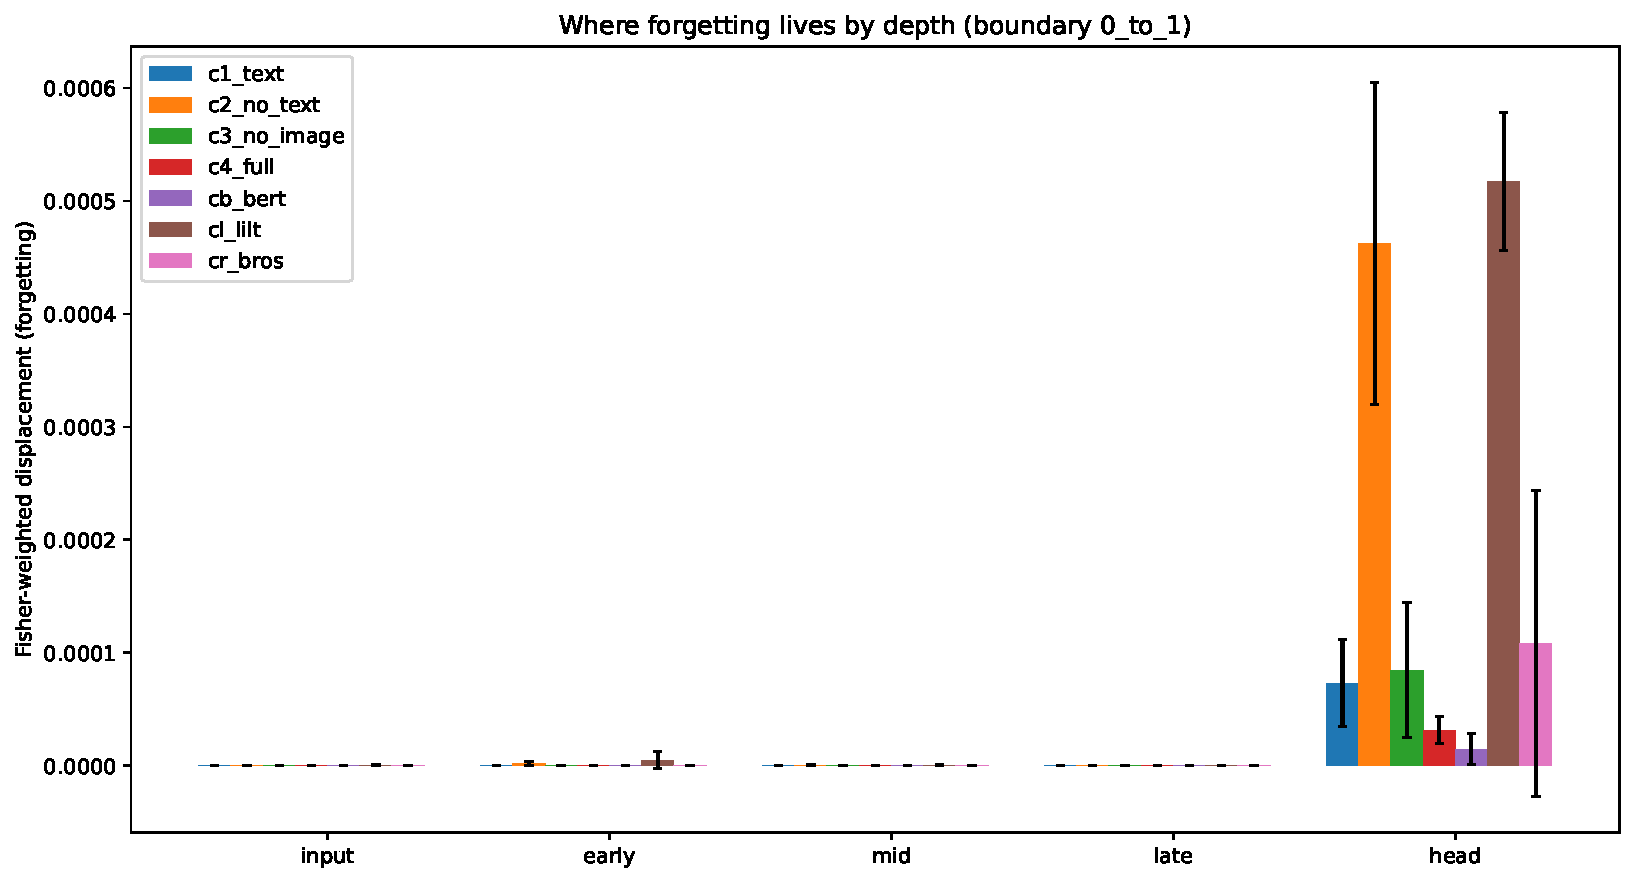
\includegraphics[width=0.92\linewidth]{figures/pilot_displacement_bars.pdf}
\caption{Where forgetting lives. Old-task-Fisher-weighted displacement $D_g$ by depth bucket (log scale, first boundary), for the four LayoutLMv3 modality-mask conditions, text-only BERT, LiLT and BROS; mean over three seeds, $\pm$1 s.d. The classifier head's weighted displacement is one to four orders of magnitude above any encoder layer's on every backbone.}
\label{fig:displacement}\end{figure}
\paragraph{Finding 1: output-localised.} Two instruments agree. Per-token CKA between consecutive checkpoints falls monotonically with depth: $1.00$ at the text/layout/patch embeddings, $0.78$ over early encoder layers, $0.34$ mid, $0.25$ at the last layer and $0.16$ at the classifier. Old-task-Fisher-weighted displacement $D_g$ (Fig.~\ref{fig:displacement}) is one to four orders of magnitude larger at the head than at any encoder bucket, on all four modality-mask conditions of LayoutLMv3, on BERT, LiLT and BROS. A per-component test rejects the null of uniform displacement with the head dominant ($p<0.01$). We separate this from Fisher \emph{importance}, which is largest at the head for any token classifier by construction ($2.2\times10^{-1}$ vs.\ $4.7\times10^{-3}$ for the next group) and is never read as forgetting. The locus is not fusion-specific: the full model (C4), text+layout (C3) and genuine text-only LayoutLMv3 (C1) forget comparably (BWT $-81$, $-88$, $-79$), so removing the visual and layout streams barely changes the profile; forgetting is carried by the text-and-head path common to all three. The text stream is the one that supports usable optimisation at all---with text removed, two of three seeds collapse to an all-background predictor.

\paragraph{Finding 1$'$: architecture-general.} Permuting LiLT's and BROS's per-depth displacement profiles against the LayoutLMv3 reference fails to reject a shared \emph{location} ($p=0.38$, $0.51$), and BERT reproduces the same head-dominant, depth-monotone pattern. We claim only shared location: at three seeds a cross-backbone comparison of forgetting \emph{magnitude} is underpowered, and we do not read the small differences in AA or BWT between backbones as meaningful.

\paragraph{Finding 2: protecting the locus relocates the drift.} If forgetting lives at the head and late layers, the natural intervention is to protect them. On DIL/LayoutLMv3 (seed 42) freezing everything after task~1 gives AA $41.1$, BWT $-0.0$: nothing is forgotten and nothing is learned. Freezing only the diagnosed head and late layers, leaving the early and mid encoder plastic, gives AA $38.8$ with BWT $-76.8$---naive-level forgetting---while early/mid CKA, which is $\approx1.0$ under naive training, collapses to $0.19$. The drift did not disappear; it migrated to whatever remained plastic. A control that adds a memory to the frozen locus without protecting it ($38.9$, $-75.6$) is indistinguishable, so drift, not the absence of a memory, is the bottleneck. This is why uniform protection fails too: a depth-scaled consolidation penalty spread equally across every bucket collapses to $42.6$ AA (it cannot fit the tasks), whereas the same budget concentrated on the head/late locus recovers $84.7$, and head-only ($86.1$) or late-only ($86.2$) each recover essentially all of it (three seeds). We read this as a conservation statement: under architectural constraint the total forgetting is redistributed, not removed. Finding~2 is established on DIL with LayoutLMv3 (seed~42 for the freeze arms, three seeds for the consolidation probe); its extension is in Appendix~\ref{app:extra}.

\paragraph{Prediction.} The anatomy is output-facing and conserved under constraint. It therefore predicts that (i) only a mechanism that re-grounds the head on old-task targets can recover competence, (ii) parameter-space protection---however placed---cannot, and (iii) the ordering should transfer across backbones because the locus does. The next three sections test each.

\section{The Anatomy Predicts the Remedy Ordering}
\label{sec:benchmark}
Table~\ref{tab:grid} reports the six classical strategies on four backbones and three scenarios, three seeds each; 68 of 72 cells are complete, and the 4 missing cells are marked rather than imputed.\footnote{The missing cells (LwF on LiLT; EWC on LiLT/CIL-CORD) exceeded the memory of the 6\,GB GPU that ran the secondary-backbone grid, even with mixed precision; they are reported as missing rather than imputed.}

\begin{table}[t]
\centering\small
\caption{Generality grid: average accuracy (mean $\pm$ s.d., three seeds) of the six classical strategies on four backbones and three scenarios. Joint is the pooled-data oracle. Grey cells did not fit the available GPU memory (see text). Replay reaches the joint bound on DIL on every backbone; regularisation and distillation stay near the naive floor; on CIL-CORD every method, replay included, sits near the floor.}
\label{tab:grid}
\setlength{\tabcolsep}{4pt}
\resizebox{\linewidth}{!}{%
\begin{tabular}{llcccccc}
\toprule
Scenario & Backbone & Naive & Joint & EWC & LwF & ER & DER++ \\
\midrule
\multirow{4}{*}{DIL}
 & LayoutLMv3 & $41.3{\pm}1.5$ & $88.7{\pm}1.1$ & $41.2{\pm}1.1$ & $43.7{\pm}1.1$ & $87.9{\pm}1.4$ & $88.0{\pm}0.9$ \\
 & LiLT       & $40.1{\pm}0.5$ & $83.8{\pm}1.2$ & $48.4{\pm}5.9$ & \cellcolor{gray!25}-- & $85.7{\pm}0.5$ & $84.4{\pm}0.3$ \\
 & BROS       & $40.3{\pm}1.8$ & $87.5{\pm}1.3$ & $45.0{\pm}4.9$ & $35.2{\pm}3.1$ & $87.8{\pm}0.4$ & $87.6{\pm}1.1$ \\
 & BERT       & $39.4{\pm}0.3$ & $77.2{\pm}0.4$ & $46.6{\pm}3.0$ & $40.5{\pm}0.1$ & $77.1{\pm}1.0$ & $77.4{\pm}0.6$ \\
\midrule
\multirow{4}{*}{CIL-CORD}
 & LayoutLMv3 & $19.0{\pm}0.2$ & $33.3{\pm}0.3$ & $0.5{\pm}0.6$ & $18.8{\pm}0.2$ & $16.0{\pm}1.4$ & $18.2{\pm}0.3$ \\
 & LiLT       & $19.1{\pm}0.3$ & $32.4{\pm}0.4$ & \cellcolor{gray!25}-- & \cellcolor{gray!25}-- & $17.9{\pm}0.5$ & $18.0{\pm}1.0$ \\
 & BROS       & $19.2{\pm}0.1$ & $32.9{\pm}0.0$ & $17.3{\pm}0.8$ & $23.1{\pm}1.2$ & $18.3{\pm}1.5$ & $17.7{\pm}1.1$ \\
 & BERT       & $19.3{\pm}0.1$ & $32.4{\pm}0.2$ & $17.9{\pm}0.3$ & $24.3{\pm}0.3$ & $17.1{\pm}1.6$ & $19.2{\pm}1.9$ \\
\midrule
\multirow{4}{*}{Mixed}
 & LayoutLMv3 & $33.9{\pm}0.3$ & $67.5{\pm}0.8$ & $22.0{\pm}9.4$ & $35.2{\pm}1.2$ & $60.3{\pm}5.3$ & $60.8{\pm}2.7$ \\
 & LiLT       & $30.7{\pm}0.7$ & $61.8{\pm}0.6$ & $28.1{\pm}3.0$ & \cellcolor{gray!25}-- & $57.0{\pm}1.4$ & $55.1{\pm}2.9$ \\
 & BROS       & $33.9{\pm}0.4$ & $65.3{\pm}2.1$ & $37.4{\pm}3.3$ & $34.4{\pm}0.5$ & $61.1{\pm}1.4$ & $63.0{\pm}0.4$ \\
 & BERT       & $23.4{\pm}0.3$ & $55.0{\pm}0.6$ & $28.6{\pm}0.9$ & $29.4{\pm}4.2$ & $50.2{\pm}0.6$ & $50.7{\pm}1.3$ \\
\bottomrule
\end{tabular}}
\end{table}

\paragraph{Replay re-grounds the head and reaches the oracle on DIL, on every backbone.} ER and DER++ reach $87.9$ and $88.0$ against the joint bound of $88.7$ on LayoutLMv3, $87.8$/$87.6$ vs.\ $87.5$ on BROS, $77.1$/$77.4$ vs.\ $77.2$ on BERT, and $85.7$/$84.4$ vs.\ $83.8$ on LiLT,\footnote{On LiLT the replay methods exceed the pooled-data oracle on all three seeds; joint training on the LiLT backbone appears to be slightly under-fitted by the shared early-stopping rule. We report it as measured.} with backward transfer of $-1$ to $-3.5$. The backbone sets the level; replay closes the gap on all of them. On Mixed, replay closes most of the gap ($60.3$--$63.0$ against oracles of $65$--$68$ on the three layout-aware backbones; $50.2$/$50.7$ vs.\ $55.0$ on BERT) with BWT around $-22$ to $-35$: the class-incremental transitions inside the sequence are where the residual forgetting sits.

\paragraph{Parameter-space protection does not.} EWC and LwF remain at the naive floor on DIL for LayoutLMv3 ($41.2$, $43.7$ vs.\ $41.3$). Both mechanisms act on parameters or on whole-network outputs; neither places an old-task gradient on the head, and the anatomy says that is the only place it would matter. EWC's Fisher penalty, computed at the head-dominant locus, does reduce backward transfer ($-2.8$ vs.\ $-73$ for naive on LayoutLMv3) but at the cost of not fitting the new tasks---the same under-fitting mode as the uniform consolidation probe of \S\ref{sec:anatomy}.

\begin{figure}[t]\centering
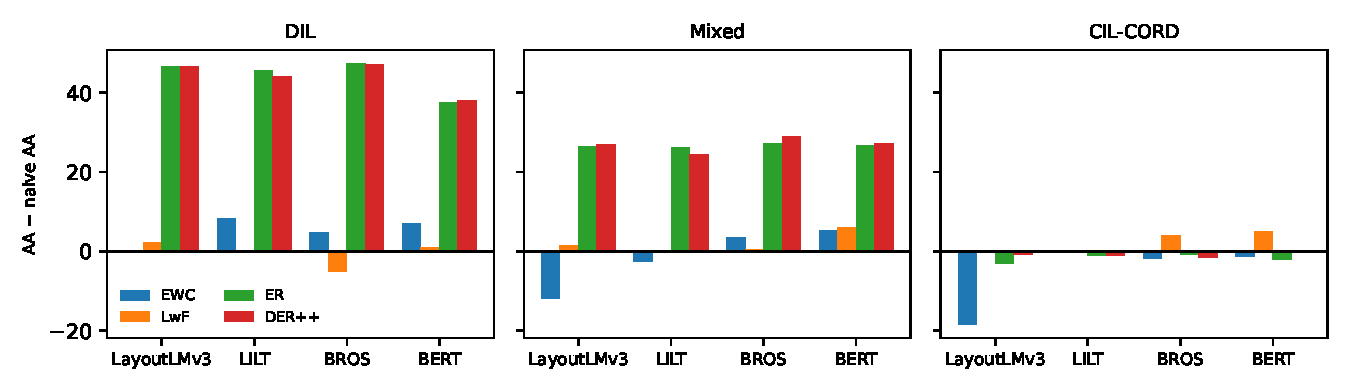
\includegraphics[width=0.95\linewidth]{figures/remedy_benefit.pdf}
\caption{Remedy benefit is backbone-dependent; the phenomenon is not. Change in AA over naive for each classical remedy, per backbone and scenario (mean of three seeds). Replay's benefit is large and consistent; EWC and LwF change sign across backbones (missing bars: cells not run).}
\label{fig:signflip}\end{figure}
\paragraph{A remedy's benefit is backbone-dependent; the phenomenon is not.} Where the naive-to-joint gap agrees to $2.5$ points across backbones on Mixed, EWC's benefit over naive spans a $17$-point range with a sign flip: $-11.8$ on LayoutLMv3, $-2.6$ on LiLT, $+3.5$ on BROS, $+5.3$ on BERT (Fig.~\ref{fig:signflip}). LwF likewise helps CIL-CORD on BROS and BERT ($+4$, $+5$) and nothing on LayoutLMv3. A single-backbone comparison of buffer-free remedies can therefore land on either side of zero; a multi-backbone protocol is not optional for this class of claims.

\paragraph{CIL-CORD is a floor regime for everyone.} With six fine-grained classes per session over a single receipt domain, every method---replay included---sits at $16$--$24$ AA against an oracle of $33$, and on LayoutLMv3 EWC collapses to $0.5$. Replay does not recover CIL-CORD with a 200-document buffer, and we report that rather than restrict the headline to DIL. The reason is the moving ``O'' boundary: what must be re-grounded is not a fixed head but a head whose background class is redefined at every session, and replayed documents carry the \emph{old} labelling of the new classes.\footnote{This is the setting in which the continual-NER literature's distillation/pseudo-labelling protocols are designed to operate; we deliberately do not engineer the O-shift away.}

\section{Falsification: Five Buffer-Free Families}
\label{sec:falsification}
Sections~\ref{sec:anatomy}--\ref{sec:benchmark} say replay works because it re-exercises the head on old-task targets. The strongest way to test that reading is to try to get the same effect without a buffer. We built or ported five buffer-free families spanning the mechanisms the literature offers, ran each on DIL/LayoutLMv3, and root-caused each failure (Table~\ref{tab:ledger}). None is a contribution; each is a witness.

\begin{table}[t]
\centering\small
\caption{Falsification ledger, DIL/LayoutLMv3 (naive floor $41.3$, replay $\approx88$). Each family is the strongest instance we could build of its mechanism; the failure reason is from a per-boundary root-cause analysis, not inferred from the score. $^\dagger$run at a frozen-backbone/3-epoch operating point (see text).}
\label{tab:ledger}
\setlength{\tabcolsep}{4pt}
\resizebox{\linewidth}{!}{%
\begin{tabular}{llcl}
\toprule
Family & Instance & Best AA & Why it fails \\
\midrule
Weight merging & TIES/Fisher head merge$^\dagger$ & $21.6$ (no-merge $21.9$) & merge of head vectors cancels; near no-op \\
Merge + realignment & LCA~\citep{lca2026} (ported) & $41.9$ & backbone merge halves BWT; Gaussian realignment kills acquisition \\
Subspace transfer & HGT / CUBER (ported) & \vnum{--} & protected subspace grows; head unconstrained \\
Parametric slots & LexSlot (no buffer) & $42.2$ & isolated head slots cannot re-ground shared head \\
Input-anchored memory & Ledger$^\dagger$ & FUNSD $21$ / SROIE $23$ & own-vs-cumulative gap is training-free \\
Feature-Gaussian replay & LexMem v3b (positive control) & $66.0$ & partial: recovers dense-label tasks only \\
 & LexMem v5 (+relational) & $63.2$; mid-task $13.0$ & marginal summary breaks doc consistency \\
\bottomrule
\end{tabular}}
\end{table}

\paragraph{One mechanism.} A per-boundary root-cause analysis of the failing methods (modality-ablated evaluation, per-class F1, token confusion, Fisher displacement) localises the failure to the readout. At the first boundary the head's output marginal on old tasks snaps to the just-trained task's gold-label marginal (cosine $0.997$--$0.998$ for naive and LwF, vs.\ $0.60$ to the old task's own marginal); replay methods stay at $0.99$--$1.00$ to their own. Classes never re-exercised (\textsc{key}, \textsc{header}) are extinguished to exactly $0.0$ F1 under every modality mask, and the background class collapses too (row accuracy $0.00\%$, invisible to entity F1). Trunk displacement is front-loaded and functionally minor. Forgetting here is a \emph{readout-marginal snap on a class-asymmetric substrate}, not representation erasure---which is exactly why every family that leaves the head un-exercised fails, and why the feature-Gaussian family, the field's strongest exemplar-free tool~\citep{zhu2021pass,petit2023fetril,goswami2023fecam}, only partially recovers: it re-exercises the head, but on marginal summaries that no longer respect what the head was trained to read (\S\ref{sec:buffer}).

\paragraph{Cheap corrections are registered nulls.} If the snap were a mis-calibrated prior, eval-time or marginal-level correction should reverse it. Five kill-tests registered with explicit support/kill bars before any run---marginal matching, prior-ratio correction, per-document EM re-estimation, a KL anchor to the prior-task label mixture, balanced-softmax logit adjustment---recover at best $-0.1$ AA and leave the extinguished classes at $0.0$ F1. A saturation probe explains why: old-class probability mass is $\sim10^{-6}$, two to three orders below the branch threshold; the information is destroyed before any correction can act. The snap is a symptom, not an invertible transform.

\paragraph{The under-training objection.} Two of the seven rows ($\dagger$) were reached at a low operating point (frozen backbone, three epochs; at-learning F1 $\approx21$ vs.\ replay's $88$). We keep them because their failure is independent of the operating point---head merging is a near no-op on strong heads too, and the ledger's own-vs-cumulative gap is training-free---but we do not rest the negative result on them. LCA, LexSlot and both LexMem rows were run at the full protocol, and they are the rows that carry the claim.

\section{What the Buffer Must Contain}
\label{sec:buffer}
If only replay works, what about replay is load-bearing? We answer with a falsification ladder over \emph{latent} replay: activations banked at a frozen encoder boundary (layer $k$) and replayed through the plastic upper layers and head, so that storage content can be varied while the mechanism is held fixed (DIL/LayoutLMv3; single-seed diagnostic runs except where noted).

\paragraph{Whole documents retain; every summary collapses.} Replaying the real banked activations of 50 whole documents per task retains AA $87.3$ (converged, $k{=}4$). Summaries of the \emph{same} store collapse to the naive level: a rank-16 spectral summary $41.9$, per-class full-dimensional Gaussians $39.4$, and even real $k$-means centroids of the banked activations $36.7$--$39.7$---so the failure is not synthesis fidelity. The single-variable control isolates the ingredient: four whole replayed documents retain $63.8$ at a matched five-epoch budget, while the identical features pasted onto decoupled layout carriers retain $36.7$. The intact (feature, position, label) binding of a document is worth $+27$ AA by itself. With five whole documents per task the small-buffer point is $66.5\pm3.0$ over three seeds.

\begin{figure}[t]\centering
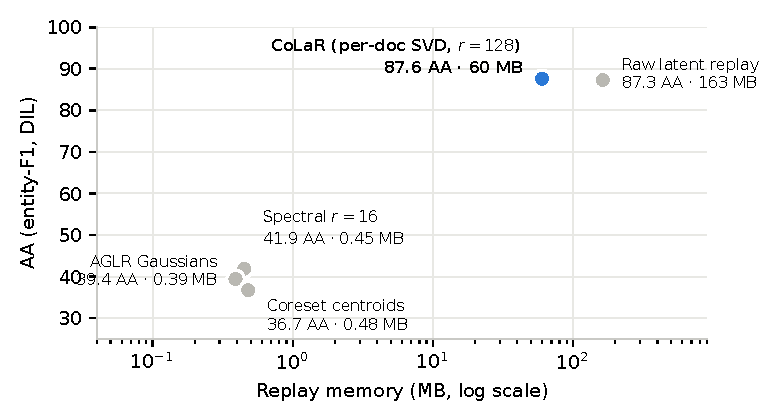
\includegraphics[width=0.7\linewidth]{figures/colar_pareto.pdf}
\caption{Replay memory versus retention (DIL, log-scale memory). Per-document SVD replay (CoLaR) matches raw latent replay at $2.7\times$ less storage because it preserves whole-document binding; every aggressive summary at ${\sim}0.4$\,MB breaks that binding and collapses to the naive level.}
\label{fig:pareto}\end{figure}
\paragraph{The constructive control.} The negatives could be effort-limited. CoLaR shows they are not: individual documents \emph{are} low-rank even though the pooled feature space is not, so per-document rank-$r$ SVD factors respect whole-document binding. At $r{=}128$ CoLaR retains AA $87.6$ (final row $[89.2, 76.3, 97.2]$ on FUNSD/SROIE/CORD; $86.8$ over three seeds) at $60$\,MB, $2.7\times$ smaller than raw latent replay at equal document count ($87.3$ at $163$\,MB) and within $1.1$ points of the oracle; $r{=}64$ gives $80.6$ at $32$\,MB (Fig.~\ref{fig:pareto}). Compression that respects the consistency law is lossless; every marginal summary is not. CoLaR is a control, not a proposed method: attempts to improve it obey a conservation law---class-balanced losses ($87.1$), coverage-based selection ($86.8$), their combination ($87.3$), entity-weighted compression ($87.1$) all trade FUNSD for SROIE about $1{:}1$ without moving AA, and a three-seed check finds no lever beats the base ($87.8$ base $=$ balanced $87.8$ $>$ $k$-centre $87.0$). Read-side extensions are clean negatives (a $k$NN readout blend is inert at $\lambda{=}0.3$ and destructive at $\lambda{=}1$, $46.2$; metaplastic consolidation is dose-dependently harmful, $85.9\rightarrow79.5$), consistent with the root cause: the readout must be repaired by re-exercise, not averaged with a weaker reader or stiffened.

\paragraph{A bounded positive on the storage side.} Replaying pseudo-labelled \emph{public} documents through the same mechanism (zero private bytes) recovers dense-label tasks (FUNSD $76.1$) but not a task whose feature region the proxy pool does not cover (SROIE $\sim7$), topping out at $58.9$: coverage-limited partial transfer, which sharpens rather than escapes the law. Budget-adaptive allocation of documents and rank across tasks moves along a Pareto frontier rather than beyond it (Appendix~\ref{app:extra}).

\section{Limitations and Implications}
\label{sec:limitations}
\paragraph{Scope of each claim.} Finding~1 (location) rests on four backbones, three seeds, and two independent instruments; its magnitude comparison across backbones is underpowered and not claimed. The benchmark ordering (\S\ref{sec:benchmark}) is three seeds on 68 of 72 cells; the missing cells are disclosed, not imputed, and none of them is a replay cell on DIL, where the headline lives. Finding~2 (migration) and the buffer-content ladder (\S\ref{sec:buffer}) are seed-42 DIL/LayoutLMv3 diagnostics with three-seed checks only at the points stated; we present them as mechanism evidence, not as generality claims. Task order matters (reversing DIL reduces naive BWT from $-81$ to $-75$) and all single-order results carry that caveat.

\paragraph{What we do not claim.} No method here is proposed. The falsified families are the strongest instances we could build, not exhaustive; a buffer-free mechanism that re-exercises the head on inputs preserving whole-document binding would be consistent with our account, and we would welcome it. CIL-CORD is a floor regime in which the O-tag shift dominates, and we have not tested whether the continual-NER distillation protocols recover it. Forward transfer is not reported because the zero-shot term is uninformative under label growth. FUNSD and SROIE lack validation splits, so early stopping on those tasks reads the evaluation set; the bias is shared by every method and bounded by patience~2.

\paragraph{Implication.} For document understanding, the research question this evidence supports is not ``how to avoid the buffer'' but ``how small can it be, and what must it hold''. The answer so far: small---tens of megabytes of per-document SVD factors---but it must hold whole documents.

\bibliography{refs}
\bibliographystyle{iclr2027_conference}

\appendix
\section{Setup details}
\label{app:setup}

\paragraph{DIL unified schema.} A single four-entity label space \{HEADER, KEY, VALUE, OTHER\} (9 BIO tags) is held fixed over FUNSD$\rightarrow$SROIE$\rightarrow$CORD. FUNSD: HEADER$\rightarrow$HEADER, QUESTION$\rightarrow$KEY, ANSWER$\rightarrow$VALUE. SROIE: COMPANY$\rightarrow$KEY; ADDRESS/DATE/TOTAL$\rightarrow$VALUE. CORD: menu/sub\_total/total$\rightarrow$VALUE; void\_menu/sub$\rightarrow$OTHER. KEY originates only from FUNSD and SROIE, so the schema is VALUE-dominant; we report per-class F1 for every DIL result and treat a high aggregate as retention only if the sparse classes are retained. The reverse order is used as a robustness check.

\paragraph{CIL-CORD sessions.} CORD's 30 fine-grained classes in five sessions of six, ordered easy-to-hard by super-class: (0) core menu fields; (1) extended menu + sub; (2) sub\_total fields; (3) total / payment methods; (4) residual total + void/auxiliary. Every receipt containing at least one in-session entity is kept, with out-of-session tokens relabelled to ``O'', giving per-session training pools of 800/382/549/723/780 receipts. Class imbalance across sessions is deliberately left unmodified. Joint uses the full-label pool (each receipt once with all its labels) rather than the concatenation of the masked per-session copies, which would feed conflicting labels for the same document.

\paragraph{Mixed.} Six sessions: CORD-menu $\rightarrow$ FUNSD $\rightarrow$ CORD-menu-extended $\rightarrow$ SROIE $\rightarrow$ CORD-sub\_total $\rightarrow$ FUNSD-revisit; boundaries alternate new-class and new-domain transitions and the final session is an explicit retention check.

\paragraph{Datasets.} FUNSD (\texttt{nielsr/funsd-layoutlmv3}; 149/50), CORD (\texttt{naver-clova-ix/cord-v2}; 800/100/100), SROIE (\texttt{mp-02/sroie}; 626/347). Dataset-provided OCR and boxes throughout; images 224$\times$224; sequence length 512.

\paragraph{Hyperparameters.} AdamW, lr $5\times10^{-5}$ constant, weight decay $0.01$, clipping $1.0$, batch size 8 on the primary grid (1--2 with gradient checkpointing on the 6\,GB secondary-backbone machine; replay batch 2, or 1 for DER++ on BROS, whose HF implementation lacks checkpointing). EWC $\lambda{=}10^3$, Fisher over 200 documents; LwF $T{=}2$, $\alpha{=}1$; ER/DER++ buffer 200 documents, DER++ $\alpha{=}\beta{=}0.5$. Early stopping on task val F1, patience 2, $\delta{=}0.1$, cap 100 epochs (never binding; tasks converge in 4--8). Seeds 42/7/123. Primary-grid runs used bf16 autocast on a 24\,GB GPU; the secondary-backbone cells ran in fp32 or fp16 on a 6\,GB GPU.

\paragraph{Compute.} Every run fits a single GPU; the full generality grid is roughly 200 GPU-hours on a 24\,GB card.

\section{Additional results}
\label{app:extra}
\todo{Per-backbone BWT/AF tables (from \texttt{results/table\_backbone\_BWT.tex}); prompt/LoRA/C-Flat++ baselines on LayoutLMv3; Finding~2 extension; PLaR sweep; CoLaSlot gates.}

\paragraph{Budget-adaptive allocation is a frontier, not a gain.} Allocating a fixed compressed-replay budget unevenly across tasks (documents $[18,5,2]$, ranks $[64,128,64]$ vs.\ a uniform $10$ documents at rank $64$; 5 epochs, $k{=}4$) gave $+4.0$ AA on seed 42 while passing a pre-registered per-domain guard. On seeds 7 and 123 the same comparison gave $-8.0$ and $+5.7$: $+0.6\pm7.5$ over three seeds, a null. The seed-42 result was a point on a Pareto frontier (old-domain retention traded against the final domain at $\approx9{:}1$), not a shift of the frontier, and we report it as such.

\end{document}
